\section{Teorema di Liouville sulla preservazione del \textit{volume} nello spazio delle fasi da parte della dinamica Hamiltoniana}

Consideriamo lo spazio-tempo delle fasi $ \pi (\mathcal{V}_{n+1}) $. Come abbiamo visto, esso risulta naturalmente fibrato su $ \mathcal{V}_{n+1} $. Ricordando che $ \mathcal{V}_{n+1} $ è \textit{fibrato su $ \mathbb{R} $} attraverso la proiezione al tempo assoluto $ t $, ne segue che $ \pi (\mathcal{V}_{n+1}) $ può essere riguardato come fibrato su $ \mathbb{R} $, attraverso una proiezione che continueremo a chiamare $ t $.

\begin{center}
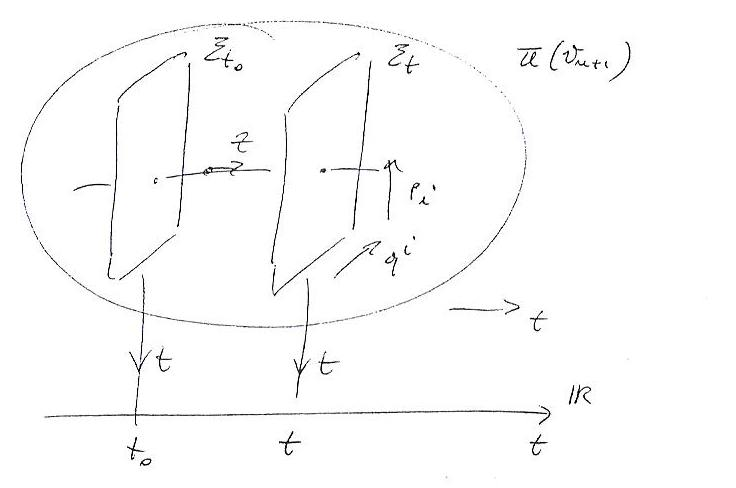
\includegraphics[width=0.65\columnwidth]{media/teorema-di-liuville-sulla-preservazione-del-volume-nello-spazio-delle-fasi-da-parte-della-dinamica-hamiltoniana/34-1.jpg}
\end{center}

indichiamo con $ \Sigma_t $ la fibra a t costante di $ t : \pi (\mathcal{V}_{n+1}) \longrightarrow \mathbb{R} $.
Evidentemente $ \Sigma_t $ costituisce una varietà differenziabile $ 2n $-dimensionale, riferibile a coordinate $ q^i, P_i$.
La dinamica Hamiltoniana, espressa dal campo vettoriale

\begin{equation*}
 Z = \frac{\partial}{\partial t} + \frac{\partial H}{\partial P_i} \frac{\partial}{\partial q^i} - \frac{\partial H}{\partial q^i} \frac{\partial}{\partial P_i}
\end{equation*}

ovvero, le curve integrali di $ Z $, stabiliscono un processo di \textit{identificazione} tra le fibre $ \Sigma_t $ a tempi diversi. In relazione al risultato (\textit{teorema di Liouville}) che vogliamo provare, risulta rilevante il fatto che le varietà $ \Sigma_t $ risultano essere dotate \textit{canonicamente di una struttura simplettica}, espressa in coordinate di $ \pi (\mathcal{V}_{n+1}) $ nella forma

\begin{equation*}
\omega = dP_i \wedge dq^i \quad \qquad \left( \sum_{i=1}^n \right) 
\end{equation*}

Da questo fatto segue che la $ 2n $-forma differenziale 

\begin{equation*}
\omega^n \stackrel{def}{=} dP_i \wedge \dots \wedge dP_n \wedge dq^1 \wedge \dots \wedge dq^n
\end{equation*}

fornisce una definizione \textit{canonica dell'elemento di volume in $ \Sigma_t $}, mediante il quale impostare un metodo \textit{intrinseco di integrazione}.

\begin{center}
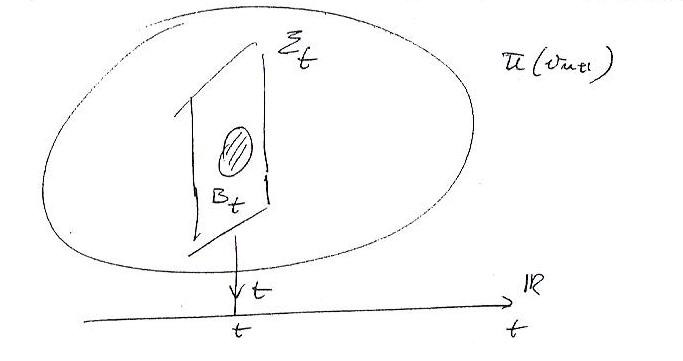
\includegraphics[width=0.5\columnwidth]{media/teorema-di-liuville-sulla-preservazione-del-volume-nello-spazio-delle-fasi-da-parte-della-dinamica-hamiltoniana/34-2.jpg}
\end{center}

Quanto detto consente di attribuire a un dominio integrabile ($ 2n $-dimensionale) $ B_t \subset \Sigma_t $ un volume

\begin{equation*}
Vol \, B_t = \int_{B_t} \omega^n = \int_{B_t} dP_i \, \dots \, dP_n \, dq^1 \, \dots \, dq^n
\end{equation*}

Ciò che è rilevante è \textit{l'intrinsecità} della valutazione data, ovvero l'indipendenza della stessa dalla scelta del sistema di coordinate.

% INIZIO PAGINA 35

Consideriamo nuovamente la dinamica \textit{Hamiltoniana} $ Z $.

\begin{center}
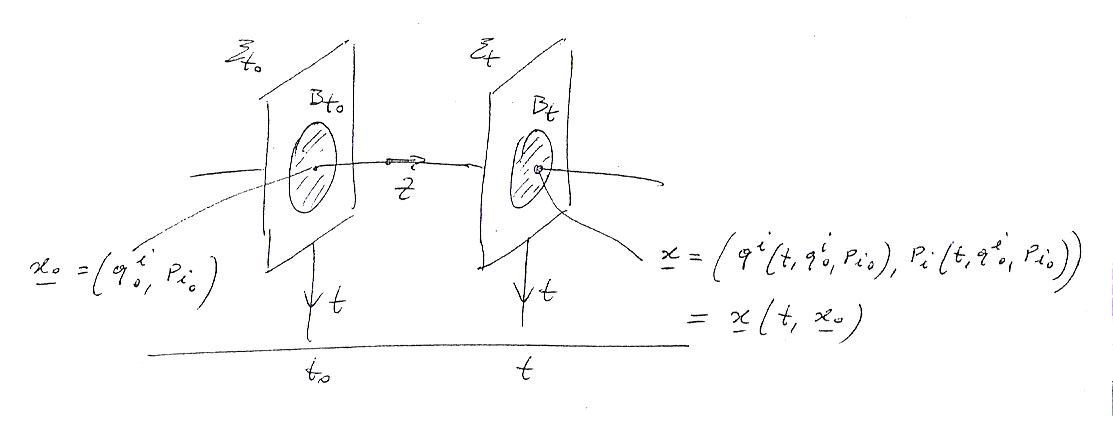
\includegraphics[width=0.95\columnwidth]{media/teorema-di-liuville-sulla-preservazione-del-volume-nello-spazio-delle-fasi-da-parte-della-dinamica-hamiltoniana/35-1.jpg}
\end{center}

Sia $ B_{t_0} $ un arbitrario dominio integrabile su $ \Sigma_{T_0} $ sia $ B_t $ ($ t $ arbitrario), il dominio che le curve integrali del vettore dinamico gli fanno corrispondere su $ \Sigma_t $.

Posto per semplicità di notazione

\begin{equation*}
\uline{x} = (\uline{P}, \uline{P}) = (q^1 \, \dots \, q^n, P_1 \, \dots \, P_n)
\end{equation*}

e indicato con

\begin{equation*}
\uline{x} = \uline{x} (t, \uline{x}_0)
\end{equation*}

le curve integrali (moti del sistema) di $ Z $, si ha

\begin{equation*}
Vol \, B_t  = \int_{B_t} dP_i \, \dots \, dP_n \, dq^1 \, \dots \, dq^n = \int_{B_t} (dx)^2n = \int_{B_{t_0}} \left| det \left( \frac{\partial \uline{x} (t, \uline{x}_0}{\partial \uline{x}_0} \right) \right| (dx_0)^{2n}
\end{equation*}

Notare che abbiamo ricondotto l'integrale nel dominio \textit{dipendente} dal tempo $ B_t $ all'integrale su un dominio \textit{fissato} $ B_0 $. Ovviamente l'integrando ora dipenderà da $ t $.
Ora, per questo fatto,

\begin{equation*}
\frac{d}{dt} Vol~B_t = \int_{B_{t_0}} \frac{\partial}{\partial t} \left| det \left( \frac{\partial \uline{x} (t, \uline{x}_0)}{\partial \uline{x}_0} \right) \right| (dx_0)^{2n}
\end{equation*}

Cominciamo a osservare che il segno di modulo è superfluo, essendo l'argomento dello stesso positivo,
Consideriamo nuovamente il campo dinamico

\begin{equation*}
 Z = \frac{\partial}{\partial t} + \frac{\partial H}{\partial P_i} \frac{\partial}{\partial q^i} - \frac{\partial H}{\partial q^i} \frac{\partial}{\partial P_i} = \frac{\partial}{\partial t} + X^i \frac{\partial}{\partial q^i} + X_i \frac{\partial}{\partial P_i}
\end{equation*}

dove

\begin{equation*}
X = X(t,\uline{x}) = \left( \frac{\partial H}{\partial P_1}, \dots ,\frac{\partial H}{\partial P_n}, \dots , -\frac{\partial H}{\partial q^1}, \dots , - \frac{\partial H}{\partial q^n} \right)
\end{equation*}

Sussiste il risultato seguente, di cui omettiamo per brevità la dimostrazione:

\begin{equation*}
\frac{\partial }{\partial t} det \left( \frac{\partial \uline{x} (t, \uline{x}_0}{\partial \uline{x}_0} \right) = \left( \sum_{\alpha = 1}^{2n} \frac{\partial X^\alpha}{\partial x^\alpha} \right) det \left( \frac{\partial \uline{x} (t, \uline{x}_0}{\partial \uline{x}_0} \right)
\end{equation*}

Osserviamo però che

\begin{equation*}
\begin{split}
\sum_{\alpha = 1}^{2n} \frac{\partial X^\alpha}{\partial x^\alpha} & = \sum_{k = 1}^{n} \frac{\partial X^k}{\partial q^k} + \sum_{k = 1}^{n} \frac{\partial X^{n+k}}{\partial P_k} = \\
& = \sum_{k = 1}^{n} \frac{\partial}{\partial q^k} \frac{\partial H}{\partial P_k} + \sum_{k = 1}^{n} \frac{\partial}{\partial P_k} \left( -\frac{\partial H}{\partial q^k}  \right) = 0
\end{split}
\end{equation*}

% INIZIO PAGINA 36

Collegando i passaggi so conclude che

\begin{equation*}
\frac{d}{dt} Vol \, B_t = 0
\end{equation*}

cioè che la dinamica Hamiltoniana preserva il volume di dominio arbitrario (integrabile) negli iperpiani $ \Sigma_t $. Questo risultato è noto come \textit{Teorema di Liouville}.
